\documentclass[a4paper, 12pt]{article}

\usepackage[T2A]{fontenc}
\usepackage[utf8]{inputenc}

\usepackage[english, russian]{babel}

\usepackage{amsmath, amsfonts, amsthm, mathtools, amssymb}
\usepackage[left = 2cm, top=10mm, right=20mm, bottom=2cm, bindingoffset=0cm]{geometry}
\usepackage{setspace}
\setstretch{1.2}
%Рисунки
\usepackage{graphicx}
\usepackage{wrapfig }
\renewcommand{\arraystretch}{1.5}

\begin{document}
\begin{titlepage}
\centering
{\scshape\LARGE Московский физико-технический институт \par}
\vspace{3cm}
{\scshape\Large Лабораторная работа № 4.4.4 \par}
\vspace{1cm}
{\huge\bfseries Интерферометр Фабри - Перо \par}
\vspace{3cm}

\vfill
\begin{flushright}
{\large выполнила студентка группы Б03-303}\par
\vspace{0.3cm}
{\LARGE Мария Шишкарёва}
\end{flushright}
\vfill

\begin{figure}[h]
 \centering
\includegraphics[width= 10 cm]{hv.png}
\end{figure}
% Bottom of the page
Долгопрудный, 2025 г.
\end{titlepage}

\large\section{Цель работы:}
определить характеристики интерферометра Фабри-Перо: база интерферометра, добротность, линейная дисперсия, аппаратная разрешающая способность.

\large\section{В работе используются:}
ртутная и натриевая лампы, интерферометры Фабри-Перо, катетометры, линзы, светофильтры, оптические скамьи

\large\section{Теория (Интерферометр Фабри-Перо):}

\begin{figure}[h]
	\begin{minipage}[h]{0.55\linewidth}
		\center{\includegraphics[width=0.95\linewidth]{ifp.png}}
	\end{minipage}
	\begin{minipage}[h]{0.5\linewidth}
		\center{\includegraphics[width=0.95\linewidth]{fp.png}}
	\end{minipage}
  \caption[]{\label{fig:ifp} Интерферометр Фабри-Перо}
\end{figure}

Интерферометр Фабри–Перо состоит из двух стеклянных (или кварцевых) пластин P1 и P2,
внутренние плоские поверхности которых
хорошо отполированы (с точностью до $10^{-2}\lambda$) и установлены параллельно друг
другу. На эти поверхности наносятся хорошо отражающие покрытия. Наружные поверхности
пластин обычно составляют небольшой угол с внутренними, чтобы световой блик,
отраженный от наружных поверхностей, не мешал наблюдениям. Интерферометр Фабри–Перо можно
рассматривать как плоскопараллельную воздушную пластину, на которой происходят
многократные отражения и интерференция световых лучей. Интерференционная картина,
наблюдаемая в фокальной плоскости линзы Л, состоит из концентрических колец равного
наклона. Для двух соседних лучей, распространяющихся между зеркалами интерферометра
под углом $\theta$, разность хода определяется соотношением
\begin{align*}
\Delta = 2L\cos\theta
\end{align*}
где $L$ --- расстояние между зеркалами.
Разрешающей способностью прибора называют величину
\begin{align*}
R = \frac{\lambda}{\delta\lambda}
\end{align*}
разрешающая способность характеризует возможность прибора различать
две близкие спектральные линии с длинами волн $\lambda$ и $\lambda+\delta\lambda$

Угловая дисперсия определяется как
\begin{align*}
D = \frac{d\varphi}{d\lambda}
\end{align*} 
По величине угловой дисперсии можно определить угловое расстояние между двумя
близкими спектральными линиями: $\delta\varphi = D\delta\lambda$

Дисперсионная область – предельная ширина спектрального интервала $\Delta\lambda$ прибора, для которой дифракционные максимумы соседних порядков не перекрываются. Она определяет диапазон
длин волн, при которых прибор может быть использоан для анализа спектра.

В случае интерферометра Фабри-Перо интерференционные
максимумы будут наблюдаться для волн, падающих под углами $\theta_{m}$, удовлетворяющими
условию:
\begin{equation}\label{max_inter}
    2L\cos{\theta_{m}} = m\lambda,
\end{equation}
где $L$ - база интерферометра. Для малых углов выражение можно переписать как 
\begin{equation}
\label{eq:1}
\theta_m^2 = 2 - \frac{\lambda}{L}m
\end{equation}
Так как  $\theta(i) = \frac{d(i)}{2f}$, где $f$ --- фокусное расстояние линзы, стоящей после интерферметра, а $d(i)$ --- диаметр i-ого кольца, можно
получить зависимость угла на максимум интерференции от его номера или диаметра кольца 
\begin{equation}
\label{eq:2}
\frac{d^2(i)}{4f^2} = \theta^2(i) = \text{const} + \frac{i\lambda}{L}
\end{equation}

Выражение можно преобразовать для получения угловой дисперсии:
\begin{equation}
    D_{\text{угл}} \approx -\frac{1}{\lambda \theta_{m}},
\end{equation}
где $\theta_{m} = \frac{d}{2f}$ в данной работе ($f$ -- фокусное расстояние используемой в работе линзы).

Также для малых углов условие возникновения  интерференционного кольца можно записать в виде:
\begin{equation}
    \frac{\lambda}{L} = \frac{1}{4f^2}\frac{\Delta(d^2_i)}{\Delta(i)},
\end{equation}

Отсюда следует используемая в работе формула для линейной дисперсии, которая используется в работе:
\begin{equation}
    D = \frac{2f^{2}}{\lambda d}
\end{equation}

Аппаратная разрешающая способность для порядка спектра $m \approx \frac{2L}{\lambda}$ может быть найдена как:
\begin{equation}
    R = \frac{\lambda}{\delta \lambda} = \frac{\pi \sqrt{r}}{1 - r}m = Nm,
\end{equation}
где $N = \dfrac{\pi \sqrt{r}}{1 - r}$ -- число интерферирующих лучей.

Дисперсионная область интерферометра Фабри-Перо может быть найдена по следующей формуле:
\begin{equation}
    \Delta \lambda = \frac{\lambda^{2}}{2L}.
\end{equation}

\large\section{Схема установки:}
В работе используются ртутная и натриевая лампы; интерферометры Фабри-Перо,
катетометры, линзы, светофильтры, оптические скамьи.
\begin{figure}[htbp]
\centerline{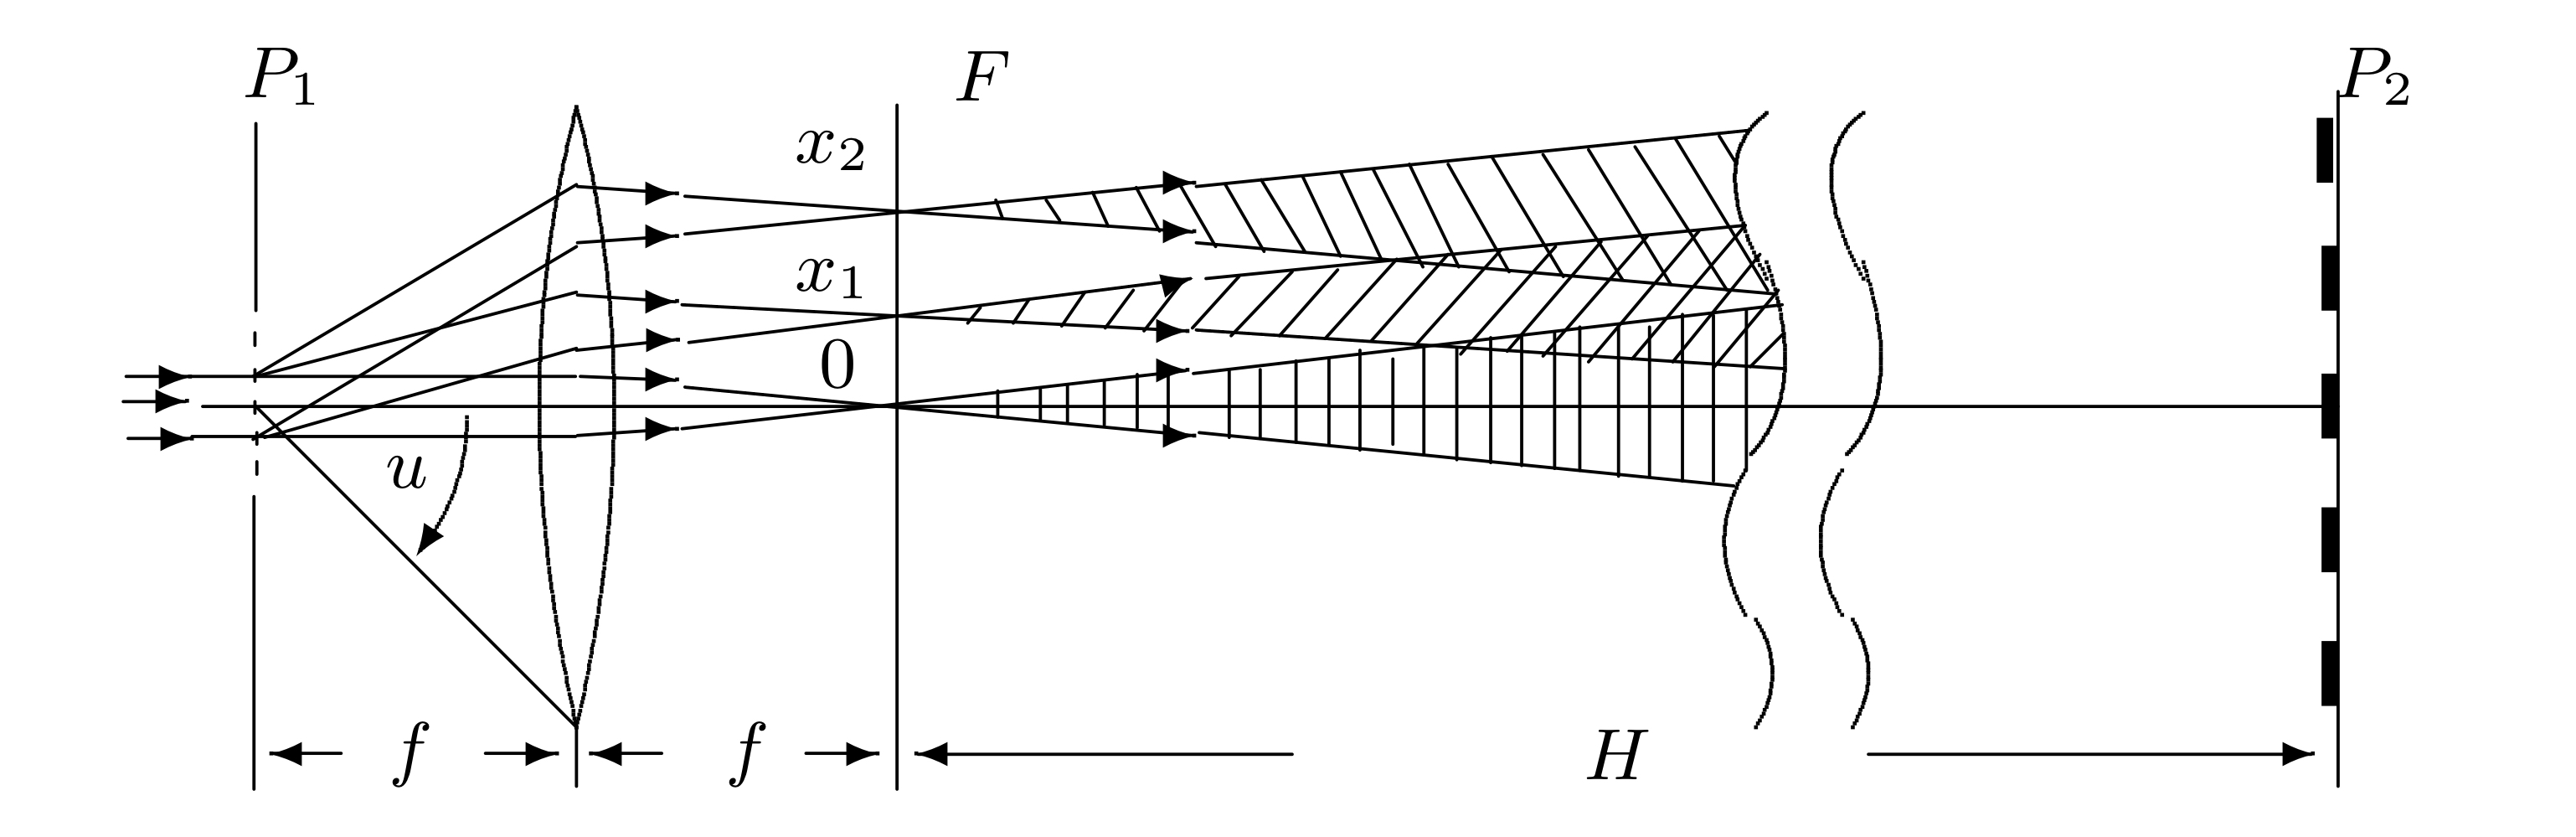
\includegraphics[width=0.7\textwidth]{ust.png}}
\caption[]{\label{fig:scheme} Схема установки}
\end{figure}

На схеме S --- лампа, $\text{Л}_{0}$ --- линза, C --- светофильтр, ИФП --- интерферометр
Фабри-Перо, T --- зрительная труба. Диаметры колец измеряются с помощью микроскопа
катетометра.

\large\section{Результаты измерений:}
\subsection{Ртутная лампа}
 погрешность катетометра $\sigma_{кат}$ = 0.02 мм
 \par
 фокусное расстояние линзы f = 50 мм

 \begin{table}[h]
 \centering
\begin{tabular}{|lll|}
\hline
\multicolumn{3}{|l|}{$\text{зелёный фильтр}$}                                               \\ \hline
\multicolumn{1}{|l|}{m} & \multicolumn{1}{l|}{$d_{\text{верх}}$, мм} & $d_{\text{низ}}$, мм \\ \hline
\multicolumn{1}{|l|}{1} & \multicolumn{1}{l|}{197.64}                 & 152.14                \\ \hline
\multicolumn{1}{|l|}{2} & \multicolumn{1}{l|}{195.95}                 & 153.56                \\ \hline
\multicolumn{1}{|l|}{3} & \multicolumn{1}{l|}{193.93}                 & 155.03                \\ \hline
\multicolumn{1}{|l|}{4} & \multicolumn{1}{l|}{191.91}                 & 156.41                \\ \hline
\multicolumn{1}{|l|}{5} & \multicolumn{1}{l|}{189.67}                 & 158.28                \\ \hline
\multicolumn{1}{|l|}{6} & \multicolumn{1}{l|}{187.23}                 & 159.95                \\ \hline
\multicolumn{1}{|l|}{7} & \multicolumn{1}{l|}{183.54}                 & 170.31                \\ \hline
\end{tabular}
\end{table}
\par

\begin{table}[h]
\centering
\begin{tabular}{|llllll|}
\hline
\multicolumn{6}{|l|}{$\text{жёлтый фильтр}$}                                                                                                                                                                                       \\ \hline
\multicolumn{1}{|l|}{m} & \multicolumn{1}{l|}{$d_{\text{верх} 1}$, мм} & \multicolumn{1}{l|}{$d_{\text{низ}1}$, мм} & \multicolumn{1}{l|}{} & \multicolumn{1}{l|}{$d_{\text{верх}2}$, мм} & $d_{\text{низ}2}$, мм \\ \cline{1-3} \cline{5-6} 
\multicolumn{1}{|l|}{1} & \multicolumn{1}{l|}{198.00}                  & \multicolumn{1}{l|}{155.90}                & \multicolumn{1}{l|}{}                  & \multicolumn{1}{l|}{197.40}                 & 156.30                \\ \cline{1-3} \cline{5-6} 
\multicolumn{1}{|l|}{2} & \multicolumn{1}{l|}{196.30}                  & \multicolumn{1}{l|}{157.59}                & \multicolumn{1}{l|}{}                  & \multicolumn{1}{l|}{195.83}                 & 158.07                \\ \cline{1-3} \cline{5-6} 
\multicolumn{1}{|l|}{3} & \multicolumn{1}{l|}{194.64}                  & \multicolumn{1}{l|}{159.31}                & \multicolumn{1}{l|}{}                  & \multicolumn{1}{l|}{193.97}                 & 159.99                \\ \cline{1-3} \cline{5-6} 
\multicolumn{1}{|l|}{4} & \multicolumn{1}{l|}{192.81}                  & \multicolumn{1}{l|}{161.21}                & \multicolumn{1}{l|}{}                  & \multicolumn{1}{l|}{192.11}                 & 161.91                \\ \cline{1-3} \cline{5-6} 
\multicolumn{1}{|l|}{5} & \multicolumn{1}{l|}{190.63}                  & \multicolumn{1}{l|}{163.57}                & \multicolumn{1}{l|}{}                  & \multicolumn{1}{l|}{191.84}                 & 164.23                \\ \cline{1-3} \cline{5-6} 
\multicolumn{1}{|l|}{6} & \multicolumn{1}{l|}{188.00}                  & \multicolumn{1}{l|}{166.15}                & \multicolumn{1}{l|}{}                  & \multicolumn{1}{l|}{186.95}                 & 167.15                \\ \cline{1-3} \cline{5-6} 
\multicolumn{1}{|l|}{7} & \multicolumn{1}{l|}{184.43}                  & \multicolumn{1}{l|}{169.82}                & \multicolumn{1}{l|}{}                  & \multicolumn{1}{l|}{182.74}                 & 171.67                \\ \hline
\end{tabular}
\end{table}
\newpage
$\delta r_{\text{зел}}$ = ((181.01 - 179.93) $\pm$ 0.02) мм = (1.08 $\pm$ 0.02) мм
\par

$\delta r_{\text{жёлт}}$ = ((182.12 - 172.35) $\pm$ 0.02) мм = (9.77 $\pm$ 0.02) мм


\subsection{Натриевая лампа}
 погрешность катетометра $\sigma_{кат}$ = 0.02 мм
 \par
 фокусное расстояние линзы f = 94 мм

\begin{table}[h]
\centering
\begin{tabular}{|llllll|}
\hline
\multicolumn{6}{|l|}{$\text{жёлтый фильтр}$}                                                                                                                                                                                       \\ \hline
\multicolumn{1}{|l|}{m} & \multicolumn{1}{l|}{$d_{\text{верх} 1}$, мм} & \multicolumn{1}{l|}{$d_{\text{низ}1}$, мм} & \multicolumn{1}{l|}{} & \multicolumn{1}{l|}{$d_{\text{верх}2}$, мм} & $d_{\text{низ}2}$, мм \\ \cline{1-3} \cline{5-6} 
\multicolumn{1}{|l|}{1} & \multicolumn{1}{l|}{174.50}                  & \multicolumn{1}{l|}{136.71}                & \multicolumn{1}{l|}{}                  & \multicolumn{1}{l|}{174.01}                 & 137.12                \\ \cline{1-3} \cline{5-6} 
\multicolumn{1}{|l|}{2} & \multicolumn{1}{l|}{173.00}                  & \multicolumn{1}{l|}{138.05}                & \multicolumn{1}{l|}{}                  & \multicolumn{1}{l|}{172.52}                 & 138.51                \\ \cline{1-3} \cline{5-6} 
\multicolumn{1}{|l|}{3} & \multicolumn{1}{l|}{171.44}                  & \multicolumn{1}{l|}{139.60}                & \multicolumn{1}{l|}{}                  & \multicolumn{1}{l|}{170.91}                 & 140.13                \\ \cline{1-3} \cline{5-6} 
\multicolumn{1}{|l|}{4} & \multicolumn{1}{l|}{169.74}                  & \multicolumn{1}{l|}{141.38}                & \multicolumn{1}{l|}{}                  & \multicolumn{1}{l|}{169.11}                 & 141.99                \\ \cline{1-3} \cline{5-6} 
\multicolumn{1}{|l|}{5} & \multicolumn{1}{l|}{167.73}                  & \multicolumn{1}{l|}{143.37}                & \multicolumn{1}{l|}{}                  & \multicolumn{1}{l|}{167.14}                 & 144.05                \\ \cline{1-3} \cline{5-6} 
\multicolumn{1}{|l|}{6} & \multicolumn{1}{l|}{165.31}                  & \multicolumn{1}{l|}{145.75}                & \multicolumn{1}{l|}{}                  & \multicolumn{1}{l|}{164.35}                 & 146.61                \\ \cline{1-3} \cline{5-6} 
\multicolumn{1}{|l|}{7} & \multicolumn{1}{l|}{162.19}                  & \multicolumn{1}{l|}{149.05}                & \multicolumn{1}{l|}{}                  & \multicolumn{1}{l|}{160.53}                 & 150.63                \\ \hline
\end{tabular}
\end{table}
\par

$\delta r_{\text{жёлт}}$ = ((160.51 - 160.27) $\pm$ 0.02) мм = (0.24 $\pm$ 0.02) мм

\large\section{обработка результатов:}
\subsection{Зелёный фильтр ртутной лампы}
Строим график зависимости $d^2(i)$ и по коэффиценту наклона находим базу L интерферометра, используя формулу (5):

\begin{figure}[h]
 \centering
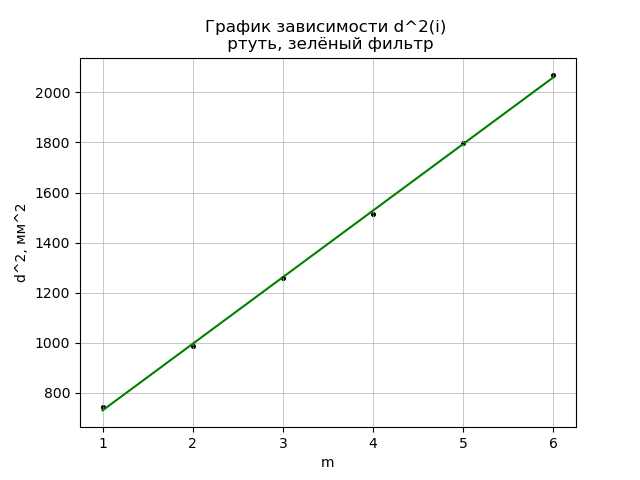
\includegraphics[width= 12 cm]{График зависимости d^2(i) для зелёного фильтра ртутной лампы.png}
\end{figure}
коэффициент наклона k = (221.01 $\pm$ 0.06) $\text{мм}^2$
\par 
$\lambda$ (Hg) = 546.10 нм
\par
L = (119.593 $\pm$ 0.062) мкм
\newpage

\subsection{Жёлтый фильтр ртутной лампы}
Строим график зависимости <d> ($\frac{1}{\Delta d}$):
\par
\begin{figure}[h]
 \centering
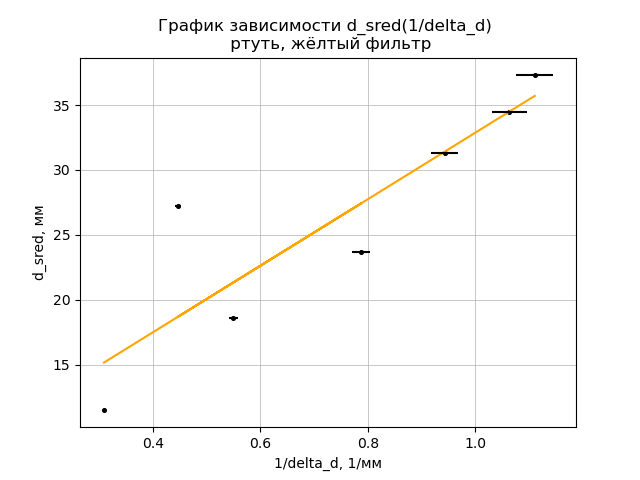
\includegraphics[width= 12 cm]{График зависимости d_sred(1delta_d) для жёлтого фильтра ртутной лампы.png}
\end{figure}
\par
коэффициент наклона k = (32.18 $\pm$ 0.74) $\text{мм}^2$ 
По коэффициенту наклона прямой находим разность длин волн $\Delta$ $\lambda$ для жёлтой пары линий ртути ($\lambda$ (Hg) = 578 нм) по формуле (5):
\par
$\Delta$ $\lambda$ = (3.84 $\pm$ 0.09) Арм


\subsection{Натриевая лампа}
Проводим аналогичные рассчёты для жёлтого света натриевой лампы
\par
$\lambda$ (Na) = 589.3 нм

\begin{figure}[h]
 \centering
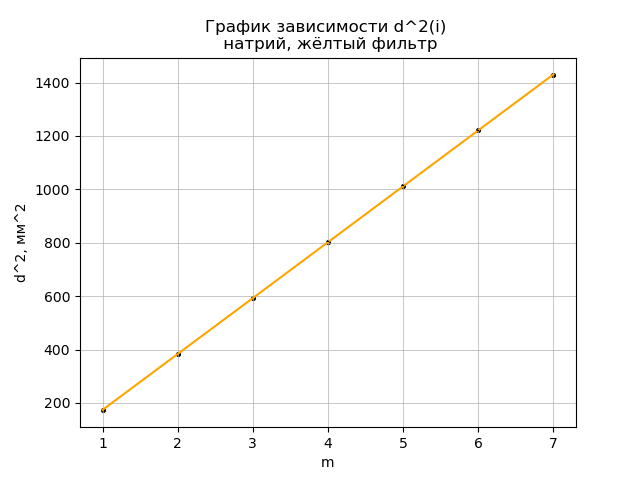
\includegraphics[width= 12 cm]{График зависимости d^2(i) для жёлтого фильтра натриевой лампы.png}
\end{figure}
\par

\begin{figure}[h]
 \centering
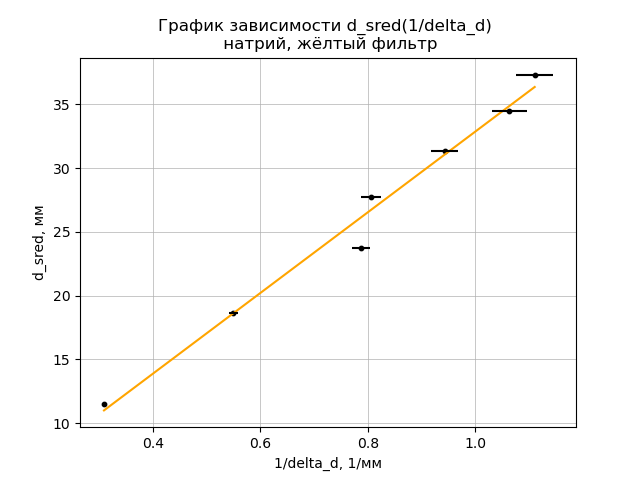
\includegraphics[width= 12 cm]{График зависимости d_sred(1delta_d) для жёлтого фильтра натриевого лампы.png}
\end{figure}

\par
$\Delta$ $\lambda$ = (5.36 $\pm$ 0.13) Арм
\par
L = (116.134 $\pm$ 0.072) мкм


\subsection{Дополнительные расчёты}
\subsubsection{Натриевая лампа}
Экспериментальное значение линейной дисперсии интерферометра:
\par
$D_{эксп}$ = (0.29 $\pm$ 0.01) $\frac{мм}{Арм}$
\par
Теоретическое значение линейной дисперсии интерферометра:
\par
$D_{теор}$ = (0.27 $\pm$ 0.05) $\frac{мм}{Арм}$
\par
Аппаратная разрешающая способность:
\par
$R_{a}$ = 8355.3 $\pm$ 2.6


\subsubsection{Ртутная лампа}
Экспериментальное значение линейной дисперсии интерферометра:
\par
$D_{эксп}$ = (0.30 $\pm$ 0.08) $\frac{мм}{Арм}$
\par
Теоретическое значение линейной дисперсии интерферометра:
\par
$D_{теор}$ = (0.39 $\pm$ 0.06) $\frac{мм}{Арм}$
\par
Аппаратная разрешающая способность:
\par
$R_{a}$ = 6101.5 $\pm$ 1.9


\large\section{Вывод:}
Были найдены характеристики интерферометра Фабри-Перо: база интерферометра, добротность, линейная дисперсия и аппаратная разрешающая способность. Результаты измерений и вычислений совпадают с теоретическими данными в пределах погрешностей


\end{document}
